
\documentclass[12pt]{article}

% Layout.
\usepackage[top=1in, bottom=0.75in, left=1in, right=1in, headheight=1in, headsep=6pt]{geometry}

% Fonts.
\usepackage{mathptmx}
\usepackage[scaled=0.86]{helvet}
\renewcommand{\emph}[1]{\textsf{\textbf{#1}}}

% TiKZ.
\usepackage{tikz, pgfplots}
\usetikzlibrary{calc}
\pgfplotsset{compat = newest}
 
\pgfplotsset{my style/.append style={axis x line=middle, axis y line=
middle, xlabel={$x$}, ylabel={$y$}, axis equal
}}

% Misc packages.
\usepackage{amsmath,amssymb,latexsym}
\usepackage{graphicx}
\usepackage{array}
\usepackage{xcolor}
\usepackage{multicol}

% Commands to set various header/footer components.
\makeatletter
\def\doctitle#1{\gdef\@doctitle{#1}}
\doctitle{Use {\tt\textbackslash doctitle\{MY LABEL\}}.}
\def\docdate#1{\gdef\@docdate{#1}}
\docdate{Use {\tt\textbackslash docdate\{MY DATE\}}.}
\def\doccourse#1{\gdef\@doccourse{#1}}
\let\@doccourse\@empty
\def\docscoring#1{\gdef\@docscoring{#1}}
\let\@docscoring\@empty
\def\docversion#1{\gdef\@docversion{#1}}
\let\@docversion\@empty
\makeatother

% Headers and footers layout.
\makeatletter
\usepackage{fancyhdr}
\pagestyle{fancy}
\fancyhf{} % Clears all headers/footers.
\lhead{\baselineskip 30pt
%\emph{\@doctitle\hfill\@docdate}
\emph{\@docdate\hfill\@doctitle}
\ifnum \value{page} > 1\relax\else\\
\emph{Name: \rule{3.5in}{1pt}\hfill \@docscoring}\fi}
\rfoot{\emph{\@docversion}}
\lfoot{\emph{\@doccourse}}
\cfoot{\emph{\thepage}}
\renewcommand{\headrulewidth}{0pt}%
\makeatother

% Paragraph spacing
\parindent 0pt
\parskip 6pt plus 1pt

% A problem is a section-like command. Use \problem{5} to
% start a problem worth 5 points.
\newcounter{probcount}
\newcounter{subprobcount}
\setcounter{probcount}{0}
\newcommand{\problem}[1]{%
\par
\addvspace{4pt}%
\setcounter{subprobcount}{0}%
\stepcounter{probcount}%
\makebox[0pt][r]{\emph{\arabic{probcount}.}\hskip1ex}\emph{[#1 points]}\hskip1ex}
\newcommand{\thesubproblem}{\emph{\alph{subprobcount}.}}

% Subproblems are an enumerate-like environment with a consistent
% numbering scheme. 
% Use \begin{subproblems}\item...\item...\end{subproblems}
\newenvironment{subproblems}{%
\begin{enumerate}%
\setcounter{enumi}{\value{subprobcount}}%
\renewcommand{\theenumi}{\emph{\alph{enumi}}}}%
{\setcounter{subprobcount}{\value{enumi}}\end{enumerate}}

% Blanks for answers in normal and math mode.
\newcommand{\blank}[1]{\rule{#1}{0.75pt}}
\newcommand{\mblank}[1]{\underline{\hspace{#1}}}
\def\emptybox(#1,#2){\framebox{\parbox[c][#2]{#1}{\rule{0pt}{0pt}}}}

% Misc.
\renewcommand{\d}{\displaystyle}
\newcommand{\ds}{\displaystyle}
\def\bc{\begin{center}}
\def\ec{\end{center}}
\def\be{\begin{enumerate}}
\def\ee{\end{enumerate}}


\doctitle{Math 251: Quiz 10}
\docdate{Apr 20, 2023}
\doccourse{UAF Calculus I}
\docversion{v-1}
\docscoring{\blank{0.8in} / 25}
\begin{document}

There are 25 points possible on this quiz. No aids (book, calculator, etc.)
are permitted.  {\bf Show all work for full credit.}

\problem{5} Find the derivatives.
\begin{subproblems}
	\item $\displaystyle G(x)=\int_0^x \sqrt{1+2t^2} \: dt$
	\vspace{0.5in}
	\item  $\displaystyle H(x)=\int_1^{x^3} 8\sin\left(\frac{1}{t}\right) \: dt$
	\vspace{0.5in}
\end{subproblems}

\problem{6} The velocity of a particle moving along a straight line is given by  $v(t)=t^2-1$ where $0 \leq t \leq 2$ is measured in seconds and $v$ is measured in meters per second. 
\begin{subproblems}
	\item Find the \emph{displacement} of the particle between $t=0$ and $t=2.$
	\vfill
	\item Find the \emph{distance traveled} of the particle between $t=0$ and $t=2.$
	\vfill
	\item Does the problem contain sufficient information to determine the position of the particle at time $t=2$? If so, determine the position. If not, explain why not. 	
	\vspace{0.5in}
\end{subproblems}


\newpage
\problem{4} Use the graph of $f(x)$ (below) to answer questions about $\displaystyle A(x)= \int_0^x f(t) \: dt.$

\begin{multicols}{2}
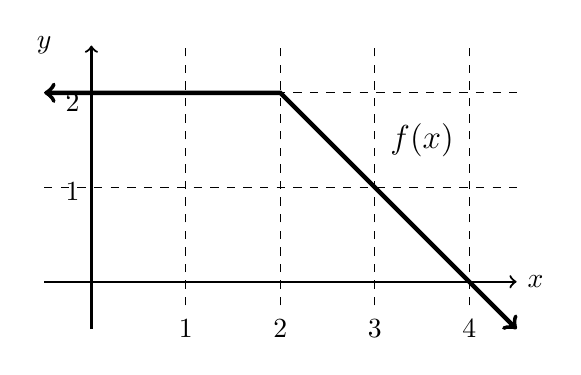
\begin{tikzpicture}[scale=1.2]
\draw[thick, ->] (-0.5,0) -- (4.5,0);
\draw[thick,->] (0,-0.5) -- (0,2.5);
\draw[ultra thick, <->] (-0.5,2) -- (2,2)-- (4.5,-0.5);
\node at (4.7,0){$x$};
\node at (-.5,2.5){$y$};
\foreach \i in {1,2,3,4}{
	\draw[dashed] (\i,-.25) -- (\i, 2.5);
	\node at (\i,-.5){$\i$};
	}
\foreach \i in {1,2}{
	\draw[dashed]  (-.5,\i) -- (4.5,\i);
	\node at (-.2,0.95*\i){$\i$};
	}
\node at (3.5,1.5){\large{$f(x)$}};
\end{tikzpicture}
\columnbreak
\begin{subproblems}
	\item $A(0)=$
	\item $A(4)=$
	\item At $x=3,$ is $A(x)$ increasing, decreasing, or neither?
\end{subproblems}
\end{multicols}

\vspace{.3in}
\problem{12} Evaluate the definite integrals below.
\begin{subproblems}
	\item $\displaystyle \int_{1}^{3} (2-6x^2)\: dx$
	\vfill
	\item $\displaystyle \int_{0}^{1} \sin (5x)\: dx$
	\vfill
	\item $\displaystyle \int_{0}^{2} \frac{x^2}{\sqrt{1+x^3}} \: dx$
	\vfill
\end{subproblems}
	
\end{document}

